\documentclass[aspectratio=169]{beamer}
\usetheme{Madrid}
\usecolortheme{default}

% Packages
\usepackage[utf8]{inputenc}
\usepackage{amsmath}
\usepackage{amsfonts}
\usepackage{amssymb}
\usepackage{graphicx}
\usepackage{listings}
\usepackage{xcolor}
\usepackage{tikz}
\usepackage{algorithm}
\usepackage{algorithmic}
\usepackage[normalem]{ulem}

% Code listing style
\lstset{
    language=C++,
    basicstyle=\tiny\ttfamily,
    keywordstyle=\color{blue},
    commentstyle=\color{green!60!black},
    stringstyle=\color{red},
    numbers=left,
    numberstyle=\tiny,
    breaklines=true,
    frame=single,
    backgroundcolor=\color{gray!10}
}

% Title page information
\title[Parallel Text Reference Breaker]{Parallel Text Reference Breaker}
\subtitle{Efficient Wikipedia Reference Detection using Aho-Corasick Algorithm and OpenMP}
\author{Rui Cai}
\institute{Parallel Programming Course Project 2025}
\date{\today}

\begin{document}

% Title slide
\frame{\titlepage}

% Outline
\begin{frame}{Outline}
\tableofcontents
\end{frame}

\section{Project Overview}

\begin{frame}{Project Overview}
\begin{itemize}
    \item \textbf{Goal}: Automatically identify and annotate Wikipedia references in large text files
    \item \textbf{Approach}: Parallel text processing using Aho-Corasick string matching algorithm
    \item \textbf{Implementation}: C++11 with OpenMP parallelization
    \item \textbf{Output}: JSON format with reference annotations and positions
\end{itemize}

\vspace{0.5cm}
\begin{block}{Key Features}
\begin{itemize}
    \item Offline Wikipedia titles database matching
    \item Parallel processing with configurable thread count
    \item Memory-efficient immutable trie structure
    \item 1KB block-based text segmentation
\end{itemize}
\end{block}
\end{frame}

\begin{frame}{Problem Statement}
\begin{columns}
\begin{column}{0.6\textwidth}
\textbf{Challenge:}
\begin{itemize}
    \item Large text files need semantic annotation
    \item Manual reference identification is time-consuming
    \item Need to match against millions of Wikipedia titles
    \item Performance requirements for real-time processing
\end{itemize}

\vspace{0.3cm}
\textbf{Solution:}
\begin{itemize}
    \item Automated reference detection
    \item Parallel processing for scalability
    \item Efficient string matching algorithm
    \item Structured JSON output format
\end{itemize}
\end{column}
\begin{column}{0.4\textwidth}
\begin{center}
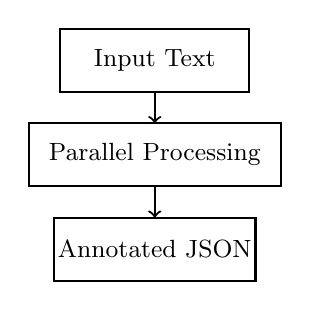
\begin{tikzpicture}[scale=0.8]
    % Input text
    \draw[thick] (0,3) rectangle (3,4);
    \node at (1.5,3.5) {\small Input Text};
    
    % Arrow down
    \draw[->, thick] (1.5,3) -- (1.5,2.5);
    
    % Processing
    \draw[thick] (-0.5,1.5) rectangle (3.5,2.5);
    \node at (1.5,2) {\small Parallel Processing};
    
    % Arrow down
    \draw[->, thick] (1.5,1.5) -- (1.5,1);
    
    % Output
    \draw[thick] (-0.1,0) rectangle (3.1,1);
    \node at (1.5,0.5) {\small Annotated JSON};
\end{tikzpicture}
\end{center}
\end{column}
\end{columns}
\end{frame}

\section{Usage and Applications}

\begin{frame}[fragile]{Usage Example}
\begin{block}{Command Line Interface}
\begin{verbatim}
# Basic usage
./text_reference_breaker wiki_titles.txt input.txt output.json

# Sequential mode (for comparison)
./text_reference_breaker wiki_titles.txt input.txt output.json --sequential

# Example with timing
time ./text_reference_breaker data/wiki_titles.txt large_text.txt result.json
\end{verbatim}
\end{block}

\begin{block}{JSON Output Format}
\begin{lstlisting}[language=json, basicstyle=\tiny\ttfamily]
{
  "text": "Coldplay had a tour concert in Helsinki in August, 2024.",
  "references": [
    { "start": 0, "end": 8, "titleIndex": 301, "title": "Coldplay" },
    { "start": 28, "end": 36, "titleIndex": 2105, "title": "Helsinki" },
    { "start": 40, "end": 46, "titleIndex": 984, "title": "August" }
  ]
}
\end{lstlisting}
\end{block}
\end{frame}

\begin{frame}{Applications and Use Cases}
\begin{block}{Academic and Research}
\begin{itemize}
    \item Automatic citation generation for research papers
    \item Content analysis and topic modeling
    \item Knowledge graph construction
\end{itemize}
\end{block}

\begin{block}{Content Management}
\begin{itemize}
    \item Wiki-style reference systems
    \item Educational content annotation
    \item News article fact-checking preparation
\end{itemize}
\end{block}

\begin{block}{Data Processing}
\begin{itemize}
    \item Large-scale text corpus analysis
    \item Information extraction pipelines
    \item Semantic text enrichment
\end{itemize}
\end{block}
\end{frame}

\section{Algorithm and Data Structures}

\begin{frame}{Aho-Corasick Algorithm}
\begin{columns}
\begin{column}{0.5\textwidth}
\textbf{Why Aho-Corasick?}
\begin{itemize}
    \item Multiple pattern matching in single pass
    \item Time complexity: O(n + m + z)
    \begin{itemize}
        \item n = text length
        \item m = total pattern length
        \item z = number of matches
    \end{itemize}
    \item Efficient for large pattern sets
    \item Immutable trie structure
\end{itemize}
\end{column}
\begin{column}{0.5\textwidth}
\begin{center}
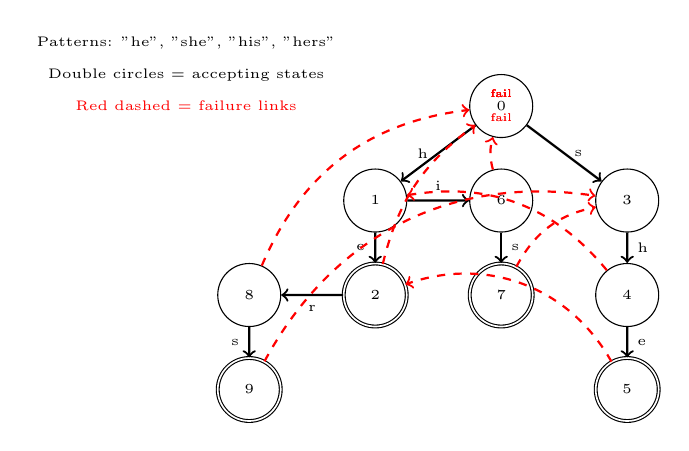
\begin{tikzpicture}[scale=0.8]
    % Define node styles
    \tikzstyle{state} = [circle, draw, minimum size=0.8cm, font=\tiny]
    \tikzstyle{accept} = [circle, draw, double, minimum size=0.8cm, font=\tiny]
    \tikzstyle{edge} = [->, thick, font=\tiny]
    \tikzstyle{failure} = [->, dashed, red, thick, font=\tiny]
    
    % Nodes - building trie for patterns: "he", "she", "his", "hers"
    \node[state] (0) at (0,0) {0};
    \node[state] (1) at (-2,-1.5) {1};
    \node[accept] (2) at (-2,-3) {2};
    \node[state] (3) at (2,-1.5) {3};
    \node[state] (4) at (2,-3) {4};
    \node[accept] (5) at (2,-4.5) {5};
    \node[state] (6) at (0,-1.5) {6};
    \node[accept] (7) at (0,-3) {7};
    \node[state] (8) at (-4,-3) {8};
    \node[accept] (9) at (-4,-4.5) {9};
    
    % Forward edges (trie structure)
    \draw[edge] (0) -- (1) node[midway, left] {h};
    \draw[edge] (1) -- (2) node[midway, left] {e};
    \draw[edge] (0) -- (3) node[midway, right] {s};
    \draw[edge] (3) -- (4) node[midway, right] {h};
    \draw[edge] (4) -- (5) node[midway, right] {e};
    \draw[edge] (1) -- (6) node[midway, above] {i};
    \draw[edge] (6) -- (7) node[midway, right] {s};
    \draw[edge] (2) -- (8) node[midway, below] {r};
    \draw[edge] (8) -- (9) node[midway, left] {s};
    
    % Failure links (red dashed)
    \draw[failure] (2) to[bend left=20] (0) node[midway, above] {fail};
    \draw[failure] (4) to[bend right=30] (1) node[midway, below] {fail};
    \draw[failure] (5) to[bend right=40] (2) node[midway, below] {fail};
    \draw[failure] (6) to[bend left=15] (0) node[midway, above] {fail};
    \draw[failure] (7) to[bend left=25] (3) node[midway, above] {fail};
    \draw[failure] (8) to[bend left=30] (0) node[midway, above] {fail};
    \draw[failure] (9) to[bend left=35] (3) node[midway, above] {fail};
    
    % Legend
    \node[font=\tiny] at (-5, 1) {Patterns: "he", "she", "his", "hers"};
    \node[font=\tiny] at (-5, 0.5) {Double circles = accepting states};
    \node[font=\tiny, red] at (-5, 0) {Red dashed = failure links};
\end{tikzpicture}
\end{center}
\textbf{Trie with failure links}
\end{column}
\end{columns}
\end{frame}

\begin{frame}[fragile]{Data Structures}
\begin{block}{Core Data Structures}
\begin{verbatim}
struct Reference {
    size_t start;           // Start position in text
    size_t end;             // End position in text
    size_t titleIndex;      // Index in Wikipedia titles
    std::string title;      // Matched Wikipedia title
};

struct ProcessedBlock {
    std::string text;                    // Block content
    std::vector<Reference> references;   // Found references
};

class TextProcessor {
private:
    std::unique_ptr<aho_corasick::trie> trie_;
    std::unordered_map<std::string, size_t> titleIndices_;
};
\end{verbatim}
\end{block}
\end{frame}

\section{Parallel Implementation}

\begin{frame}{Parallelization Strategy}
\begin{block}{Block-Based Parallelization}
\begin{enumerate}
    \item \textbf{Text Segmentation}: Split input into 1KB blocks
    \item \textbf{Parallel Processing}: Each thread processes independent blocks
    \item \textbf{Result Aggregation}: Combine results maintaining order
    \item \textbf{Position Adjustment}: Correct reference positions for global text
\end{enumerate}
\end{block}

\vspace{0.3cm}
\begin{center}
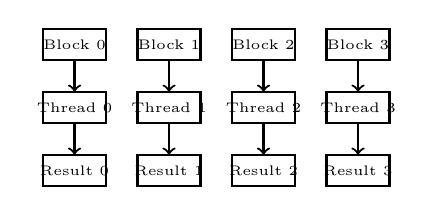
\begin{tikzpicture}[scale=0.8]
    % Input blocks
    \foreach \i in {0,1,2,3} {
        \draw[thick] (\i*1.5,2) rectangle (\i*1.5+1,2.5);
        \node at (\i*1.5+0.5,2.25) {\tiny Block \i};
    }
    
    % Threads
    \foreach \i in {0,1,2,3} {
        \draw[->, thick] (\i*1.5+0.5,2) -- (\i*1.5+0.5,1.5);
        \draw[thick] (\i*1.5,1) rectangle (\i*1.5+1,1.5);
        \node at (\i*1.5+0.5,1.25) {\tiny Thread \i};
    }
    
    % Results
    \foreach \i in {0,1,2,3} {
        \draw[->, thick] (\i*1.5+0.5,1) -- (\i*1.5+0.5,0.5);
        \draw[thick] (\i*1.5,0) rectangle (\i*1.5+1,0.5);
        \node at (\i*1.5+0.5,0.25) {\tiny Result \i};
    }
\end{tikzpicture}
\end{center}
\end{frame}

\begin{frame}[fragile]{OpenMP Implementation}
\begin{lstlisting}[caption=Parallel Processing Code]
nlohmann::json TextProcessor::processFileParallel(const std::string& inputFile) {
    std::string text = utils::readFile(inputFile);
    std::vector<std::string> blocks = splitIntoBlocks(text);
    std::vector<ProcessedBlock> processedBlocks(blocks.size());
    
    size_t currentOffset = 0;
    
    #pragma omp parallel for schedule(dynamic)
    for (size_t i = 0; i < blocks.size(); ++i) {
        size_t blockOffset = 0;
        for (size_t j = 0; j < i; ++j) {
            blockOffset += blocks[j].length();
        }
        processedBlocks[i] = processBlock(blocks[i], blockOffset);
    }
    
    return blocksToJson(processedBlocks);
}
\end{lstlisting}

\textbf{Key OpenMP Features:}
\begin{itemize}
    \item \texttt{\#pragma omp parallel for} for loop parallelization
    \item \texttt{schedule(dynamic)} for load balancing
    \item Thread-safe trie operations (read-only after construction)
\end{itemize}
\end{frame}

\begin{frame}{Performance Considerations}
\begin{columns}
\begin{column}{0.5\textwidth}
\textbf{Memory Efficiency:}
\begin{itemize}
    \item Immutable trie structure
    \item Shared read-only data
    \item Minimal memory allocation per thread
    \item Block-based processing reduces memory footprint
\end{itemize}

\vspace{0.3cm}
\textbf{Load Balancing:}
\begin{itemize}
    \item Dynamic scheduling
    \item Variable block processing times
    \item Automatic work distribution
\end{itemize}
\end{column}
\begin{column}{0.5\textwidth}
\textbf{Scalability Factors:}
\begin{itemize}
    \item Thread count = \texttt{omp\_get\_max\_threads()}
    \item No thread synchronization during processing
    \item Linear speedup potential
    \item I/O bound for very large files
\end{itemize}

\vspace{0.3cm}
\textbf{Cache Efficiency:}
\begin{itemize}
    \item Sequential block processing
    \item Locality of reference
    \item Trie fits in cache for common patterns
\end{itemize}
\end{column}
\end{columns}
\end{frame}

\section{Implementation Details}

\begin{frame}{System Architecture}
\begin{center}
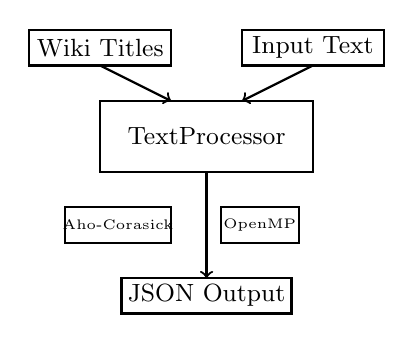
\begin{tikzpicture}[scale=0.9]
    % Input layer
    \draw[thick] (0,4) rectangle (2,4.5);
    \node at (1,4.25) {\small Wiki Titles};
    \draw[thick] (3,4) rectangle (5,4.5);
    \node at (4,4.25) {\small Input Text};
    
    % Processing layer
    \draw[thick] (1,2.5) rectangle (4,3.5);
    \node at (2.5,3) {\small TextProcessor};
    
    % Components
    \draw[thick] (0.5,1.5) rectangle (2,2);
    \node at (1.25,1.75) {\tiny Aho-Corasick};
    \draw[thick] (2.7,1.5) rectangle (3.8,2);
    \node at (3.25,1.75) {\tiny OpenMP};
    
    % Output
    \draw[thick] (1.3,0.5) rectangle (3.7,1);
    \node at (2.5,0.75) {\small JSON Output};
    
    % Arrows
    \draw[->, thick] (1,4) -- (2,3.5);
    \draw[->, thick] (4,4) -- (3,3.5);
    \draw[->, thick] (2.5,2.5) -- (2.5,1);
\end{tikzpicture}
\end{center}

\textbf{Key Components:}
\begin{itemize}
    \item \textbf{TextProcessor}: Main processing class
    \item \textbf{Aho-Corasick Trie}: Pattern matching engine
    \item \textbf{OpenMP}: Parallelization framework
    \item \textbf{JSON Output}: Structured result format
\end{itemize}
\end{frame}

\begin{frame}[fragile]{Build System and Dependencies}
\begin{block}{CMake Configuration}
\begin{verbatim}
cmake_minimum_required(VERSION 3.10)
project(text_reference_breaker VERSION 1.0)

set(CMAKE_CXX_STANDARD 11)
find_package(OpenMP REQUIRED)

Dependencies:
- nlohmann/json (JSON processing)
- aho_corasick (Header-only string matching)
- OpenMP (Parallelization)
\end{verbatim}
\end{block}

\textbf{External Dependencies:}
\begin{itemize}
    \item \textbf{Aho-Corasick}: \small{\texttt{github.com/cjgdev/aho\_corasick}}
    \item \textbf{nlohmann/json}: \small{\texttt{github.com/nlohmann/json}}
    \item \textbf{Test Data}: \small{\texttt{github.com/mmcky/nyu-econ-370}}
\end{itemize}

\textbf{Build Process:}
\begin{enumerate}
    \item Clone with submodules: \texttt{git clone --recursive}
    \item Configure: \texttt{cmake ..}
    \item Build: \texttt{make}
\end{enumerate}
\end{frame}

\section{Results and Performance}

\begin{frame}{Performance Benchmarks}
\begin{block}{Test Environment}
\begin{itemize}
    \item \textbf{Hardware}: 16-core system with OpenMP
    \item \textbf{Compiler}: GCC with C++11 and OpenMP support
    \item \textbf{Wikipedia Databases}: 51 titles vs 10,000 titles
    \item \textbf{Input Texts}: 2.2KB sample vs 3.1MB War and Peace
\end{itemize}
\end{block}

\begin{columns}
\begin{column}{0.5\textwidth}
\textbf{Small Database (51 titles):}
\begin{table}[h]
\tiny
\begin{tabular}{|l|l|r|r|}
\hline
\textbf{Input} & \textbf{Mode} & \textbf{Time} & \textbf{Speedup} \\
\hline
2.2KB & Sequential & 5.64ms & - \\
2.2KB & Parallel & 13.95ms & 0.40x \\
\hline
3.1MB & Sequential & 7863.76ms & - \\
3.1MB & Parallel & 1296.74ms & \textbf{6.06x} \\
\hline
\end{tabular}
\end{table}
\end{column}
\begin{column}{0.5\textwidth}
\textbf{Large Database (10K titles):}
\begin{table}[h]
\tiny
\begin{tabular}{|l|l|r|r|}
\hline
\textbf{Input} & \textbf{Mode} & \textbf{Time} & \textbf{Speedup} \\
\hline
2.2KB & Sequential & 1319.14ms & - \\
2.2KB & Parallel & 751.17ms & \textbf{1.76x} \\
\hline
3.1MB & Sequential & 29.4 min & - \\
3.1MB & Parallel & 4.8 min & \textbf{6.18x} \\
\hline
\end{tabular}
\end{table}
\end{column}
\end{columns}
\end{frame}

\begin{frame}{Performance Analysis}
\begin{columns}
\begin{column}{0.5\textwidth}
\textbf{Key Findings:}
\begin{itemize}
    \item \textbf{Small files}: Sequential faster (overhead dominates)
    \item \textbf{Large files}: Parallel provides 6x speedup consistently
    \item \textbf{Database scaling}: 10K titles vs 51 titles dramatically increases matches
    \item \textbf{Extreme scaling}: 29.4 min → 4.8 min for largest test (6.18x speedup)
\end{itemize}

\vspace{0.3cm}
\textbf{Reference Density Impact:}
\begin{itemize}
    \item Small text: 52 refs (51 titles) vs 3743 refs (10K titles)
    \item Large text: 193 refs (51 titles) vs 5M+ refs (10K titles)
    \item Database size directly correlates with processing time
\end{itemize}
\end{column}
\begin{column}{0.5\textwidth}
\textbf{Scalability Analysis:}
\begin{itemize}
    \item \textbf{Consistent speedup}: ~6x for large texts regardless of database size
    \item \textbf{Amdahl's Law}: Parallel portion dominates for large texts
    \item \textbf{Memory bandwidth}: Limits not reached even with 5M+ references
    \item \textbf{I/O impact}: Minimal compared to processing time
\end{itemize}

\vspace{0.3cm}
\textbf{Production Recommendations:}
\begin{itemize}
    \item Use parallel mode for files > 100KB
    \item Cache loaded databases for multiple files
    \item Expect 6x speedup for large files
    \item Balance database size vs accuracy needs
\end{itemize}
\end{column}
\end{columns}
\end{frame}

\section{Conclusion}

%\begin{frame}{Key Achievements}
%\begin{block}{Technical Accomplishments}
%\begin{itemize}
%    \item \textbf{Efficient Algorithm}: Aho-Corasick for multi-pattern matching
%    \item \textbf{Parallel Processing}: OpenMP-based scalable implementation
%    \item \textbf{Memory Efficiency}: Immutable data structures and block processing
%    \item \textbf{Production Ready}: Complete implementation with error handling
%\end{itemize}
%\end{block}
%
%\begin{block}{Software Engineering}
%\begin{itemize}
%    \item \textbf{Modern C++}: C++11 standards compliance
%    \item \textbf{Build System}: CMake with dependency management
%    \item \textbf{Documentation}: Comprehensive README and code comments
%    \item \textbf{Version Control}: Git with submodule management
%\end{itemize}
%\end{block}
%\end{frame}

\begin{frame}{Future Enhancements}
\begin{columns}
\begin{column}{0.5\textwidth}
\textbf{Performance Improvements:}
\begin{itemize}
    \item \sout{GPU acceleration (CUDA/OpenCL)}
    \item SIMD vectorization
    \item Memory-mapped I/O
    \item Distributed processing
\end{itemize}

\vspace{0.3cm}
\textbf{Feature Extensions:}
\begin{itemize}
    \item \textbf{Fuzzy matching support}
    \item Multiple language support
    \item Real-time streaming processing
    \item \textbf{Web service API}
\end{itemize}
\end{column}
\begin{column}{0.5\textwidth}
\textbf{Algorithm Enhancements:}
\begin{itemize}
    \item Context-aware matching
    \item Machine learning integration
    \item Semantic similarity scoring
    \item Disambiguation algorithms
\end{itemize}

\vspace{0.3cm}
\textbf{Scalability:}
\begin{itemize}
    \item Cloud deployment
    \item Microservice architecture
    \item Database integration
    \item Caching mechanisms
\end{itemize}
\end{column}
\end{columns}
\end{frame}

\begin{frame}{Acknowledgments}
\begin{block}{Open Source Libraries}
\begin{itemize}
    \item \textbf{Aho-Corasick Algorithm}: Header-only C++ implementation by \href{https://github.com/cjgdev}{cjgdev} \\
    \small{\texttt{https://github.com/cjgdev/aho\_corasick}}
    \item \textbf{JSON Processing}: nlohmann/json library by \href{https://github.com/nlohmann}{Niels Lohmann} \\
    \small{\texttt{https://github.com/nlohmann/json}}
    \item \textbf{OpenMP}: Parallel programming API for shared memory multiprocessing
\end{itemize}
\end{block}

\begin{block}{Data Sources}
\begin{itemize}
    \item \textbf{War and Peace Text}: Downloaded from NYU Economics 370 course materials \\
    \small{Maintained by \href{https://github.com/mmcky}{mmcky} at \texttt{github.com/mmcky/nyu-econ-370}}
    \item \textbf{Google 10K English Words}: Common English vocabulary from \href{https://github.com/first20hours/google-10000-english}{first20hours/google-10000-english} \\
    \small{Based on n-gram frequency analysis of Google's Trillion Word Corpus}
    \item \textbf{Wikipedia Titles}: Custom curated sample of 51 popular articles
\end{itemize}
\end{block}

\vspace{0.2cm}
\begin{center}
\small{Thank you to the open source community for making this project possible!}
\end{center}
\end{frame}

\begin{frame}{Questions and Discussion}
\begin{center}
\Huge Thank You!

\vspace{1cm}
\Large Questions?

\vspace{1cm}
\normalsize
\textbf{Project Repository:} \texttt{github.com/yourusername/text\_reference\_breaker}

\textbf{Technologies Used:} C++11, OpenMP, Aho-Corasick, CMake

\textbf{Key Metrics:} Parallel processing, O(n+m+z) complexity, 1KB block size
\end{center}
\end{frame}

\end{document} 